\documentclass[12pt]{article}
\usepackage{amsmath}
\usepackage{graphicx,psfrag,epsf,float, bm, subcaption}
\graphicspath{C:/Users/Colin/Documents/GitHub/BB_data_analysis/paper/fig/}
\usepackage{enumerate}
\usepackage{natbib}
\bibliographystyle{asa}
\usepackage{url} % not crucial - just used below for the URL

% no longer require relative path to figs
\graphicspath{{fig/}}

\usepackage[x11names]{xcolor}
\usepackage{framed} % provides framed env., should be removed in final draft
\definecolor{shadecolor}{rgb}{1,.5,.5}

% math macros 

\newcommand{\ind}{\stackrel{ind.}{\sim}}
\newcommand{\op}{\operatorname}
\DeclareMathOperator*{\argmin}{arg\,min}
\newcommand{\myequation}{\begin{equation}}
\newcommand{\myendequation}{\end{equation}}
\let\[\myequation
\let\]\myendequation


\pdfminorversion=4
% NOTE: To produce blinded version, replace "0" with "1" below.
\newcommand{\blind}{0}

% DON'T change margins - should be 1 inch all around.
\addtolength{\oddsidemargin}{-.5in}%
\addtolength{\evensidemargin}{-.5in}%
\addtolength{\textwidth}{1in}%
\addtolength{\textheight}{1.3in}%
\addtolength{\topmargin}{-.8in}%


\begin{document}

\def\spacingset#1{\renewcommand{\baselinestretch}%
{#1}\small\normalsize} \spacingset{1}


%%%%%%%%%%%%%%%%%%%%%%%%%%%%%%%%%%%%%%%%%%%%%%%%%%%%%%%%%%%%%%%%%%%%%%%%%%%%%%

\if0\blind
{
  \title{\bf A hierarchical failure-time model for observational data exhibiting infant-mortality and wearout failure modes}
  \author{Eric Mittman \\
    Department of Statistics, Iowa State University\\
    and \\
    Colin Lewis-Beck \\
    Department of Statistics, Iowa State University}
  \maketitle
} \fi

\if1\blind
{
  \bigskip
  \bigskip
  \bigskip
  \begin{center}
    {\LARGE\bf Title}
\end{center}
  \medskip
} \fi

\bigskip
\begin{abstract}
% Consumers have an interest in accurate assessment of product reliability.  However, lifetime data is often sparse and has limited information.  
When analyzing field data on consumer products, model-based approaches to inference require a model with sufficient flexibility to account for multiple kinds of failure. The causes of failure, while not interesting to the consumer per se, can lead to various observed lifetime distributions. Because of this, standard lifetime models, such as Weibull or lognormal may be inadequate. 
Furthermore, when the information carried by lifetime data are limited by sample size, censoring and truncation, estimates can be unstable and suffer from imprecision. These limitations are typical; for example, lifetime data for high-reliability products will naturally tend to be right-censored.


In this paper we present a method for joint estimation of multiple lifetime distributions based on the Generalized Limited Failure Population (GLFP) model. This 5-parameter model for lifetime data accommodates lifetime distributions with multiple failure modes:  early failures due to ``infant mortality'' and failures due to wearout. We fit the GLFP model using a hierarchical modeling approach.  Borrowing strength across populations, our method enables estimation with uncertainty of lifetime distributions even in cases where the number of model parameters is larger than the number of observed failures.  Moreover, using our Bayesian method, comparison of different product brands is straightforward because estimation of arbitrary functionals are easily computable using draws from the joint posterior distribution of the model parameters.
\end{abstract}

\noindent%
{\it Keywords:} GLFP, Bathtub hazard, Censored data, Hierarchical models, Bayesian estimation
\vfill

\newpage
\tableofcontents
\newpage
\spacingset{1.45} % DON'T change the spacing!
\section{Introduction}
Consumers have an interest in accurate assessment of product reliability. Toward this end, there is a need for models that can accomodate common failure patterns and methods which can make the most of available data and properly account for uncertainty.
%While computationally convenient, simple lifetime models can fail at each of these.

The reliability of many engineered products follow a similar pattern. Relatively high rates of failure occurring early (``infant mortality'') due to manufacturing defects.  After this ``burn-in'' period, failure rates stabilize as the majority of defective units have failed and are no longer in the population.  Finally, after prolonged use, rates of failure increase due to wearout.  Ignoring this pattern in failure rates can lead to suboptimal decisions and spurious inferences about a product's reliability. This highlights the importance of choosing a sufficiently flexible model.

Nonparametric methods require relatively few assumptions, but they are not suitable for forecasting. Moreover, nonparametric estimates made using small samples, or data which are heavily censored may be too noisy to be practical. Appropriate parametric models can make better use of available data. For inference, likelihood-based methods are well-equipped to deal with truncated and/or censored data. Furthermore, by assuming a parsimonious representation of the data-generating process, parametric models admit simpler, more intuitive ways to compare populations of interest, borrow strength across groups, and incorporate prior information. 

Often no information is available to identify why a unit failed and even when the failed units are available, physical failure mode analysis (sometimes referred to as ``autopsy'') can be extremely time consuming and expensive. This presents a dilemma for analysts: the data may indicate multiple failure modes, contraindicating the use of a unimodal parametric distribution. However, without any knowledge of cause of failure, traditional competing risk models are not identifiable. \citet{chan} proposed the Generalized Limited Failure Population (GLFP) model. This model can provide a solution to the problem of unknown cause of failure (masking) in the special case where there is evidence of two modes of failure which impact different stages of product life. It avoids non-identifiability by introducing a parameter representing the population proportion defective. Where this parameter is zero, the GLFP model reduces to a unimodal distribution. \\

The GLFP model has a meaningful parameterization and accommodates lifetime data with infant mortality and wearout.  Unfortunately, it can require a lot of data to fit due to the model's complexity. When multiple sources of information are available, partial pooling, accomplished via hierarchical modeling, can reduce the amount of data required to produce stable parameter estimates. When multiple populations are of interest, comparisons based on separate, unrestricted GLFP model fits will be limited to those products with sufficient data. As we will show, hierarchical modeling of the GLFP parameters allows for borrowing of information across populations which imposes ``soft'' constraints on model parameters. This enables estimation of the lifetime distribution for all populations via shrinkage toward a ``pooled" model, with the degree of shrinkage inversely related to the amount of population specific information. We demonstrate computation of various quantities of interest while comparing reliability across populations using numerical integration over the posterior distribution with samples obtained via  Markov Chain Monte Carlo. 

The structure of the paper is as follows. Section~\ref{sec:Background} introduces the proposed method and potential applications and examines previous related work in the literature.  Section~\ref{sec:GLFP model} introduces the GLFP model and illustrates its use with a subset of the Backblaze data.  In Section~\ref{sec:Data}, we describe the Backblaze Hard Drive data set, which is used throughout as a motivating example. In section~\ref{sec:Hierarchical GLFP model} we discuss using hierarchical modeling of the GLFP model parameters to extend the GLFP model to multiple populations. Section~\ref{sec:Data analysis} applies the hierarchical GLFP model to the hard disk drive data. First, we do model selection among four models of increasing complexity, using approximate leave-one-out cross-validation. Next, for the selected model, we assess the model fit using a graphical comparison of replicated data sets generated from the posterior distribution to the observed data. Finally, we present an evaluative comparison of populations taking into account practical considerations related to product lifetime. Finally, in section~\ref{sec:Discussion}, we discuss the strengths and limitations of our method and consider extensions and alternatives.

\section{Background}
\label{sec:Background}
In engineering applications, a product can often fail from one out of a set of possible malfunctioning components.  For example, a computer system can break if the mother board, disc drive or power supply stop working.  Circuit boards (CB) can fail due to a manufacturing defect or later as a result of wearout of certain components.  The general name for such products is a series system where the lifetime of the product is the minimum failure time across different components or risks \citep[Chapter 5]{nelson}.  A common assumption in series systems is the time to failure for each risk is statistically independent.  Thus, the overall reliability of a unit is modeled using the product rule across all risks.  Parameter estimation is straightforward if the cause of failure is known for each observation.  However, in many situations the cause of failure is unknown to the analyst. This is referred to in the literature as masking.\\

Previous papers have employed various data assumptions and methodologies to model masked lifetime failure data.  When modeling computer system failures \citet{reiser} assumed each observed failure came from a known subset of failure modes, and estimation was performed using a Bayesian approach.  \cite{chan} labeled the cause of circuit board failures as infant mortality, unknown, or wearout based on the time of observed failures.  This helped identify parameters when using maximum likelihood (ML) estimation.  Extending Chan and Meeker's analysis, \citet{basu} performed a Bayesian analysis with informative priors to better identify early versus late failure modes without making any assumptions about the cause of failure.  \cite{berger} introduced the Poly-Weibull distribution where cause of failure is the minimum of a several Weibull distributions.  More recently, \cite{ranjan} considered a competing risk model for infant mortality and wearout as a mixture of Weibull and exponential failure distributions.  Treating the unknown failure modes as incomplete data, an expectation maximization (EM) algorithm providing ML estimates was used, in addition to Bayesian estimation.


\section{Generalized Limited Failure Population model}
\label{sec:GLFP model}

\subsection{Weibull parameterization}
\label{sec:Weibull parameterization}
For a random variable $T$ following a Weibull distribution, the standard parameterization of the cumulative distribution function, in terms of scale parameter $\alpha$ and shape parameter $\beta$, is

$$ \Pr(T \le t) = F(t) = 1 - \exp \left[ \left( -\frac{t}{\alpha} \right)^\beta \right]. $$

An alternative parameterization, in terms of log-location parameter $\mu = \log (\alpha)$ and log-scale parameter $\sigma = 1/\beta$ is

\begin{equation} \Pr(T \le t) = F(t) = 1 - \exp \left\{ -\exp \left[ \frac{ \log (t) - \mu }{\sigma} \right] \right\}\\
= \Phi_{SEV}\left[\frac{\log (t) - \mu}{\sigma}\right],
\end{equation}
where $\Phi_{SEV}$ is the cdf of the standard smallest extreme value distribution (SEV). Thus, the Weibull distribution is a log-location scale family, with $\log(T)$ following an SEV distribution with location parameter $\mu$ and scale parameter $\sigma$. With this in mind, the corresponding density function is
\begin{equation}
f(t) =\frac{1}{\sigma t} \phi_{SEV}\left[\frac{\log(t) - \mu}{\sigma}\right]
\end{equation}

An advantage conferred by writing the model in this way is that the log of the $p$ quantile, $t_p$, is a linear function of the parameters, which allows an analyst to apply prior information in a straightforward way.  Using the inverse cdf of the SEV distribution,
\begin{equation}
\log(t_p) = \mu + \sigma \Phi_{SEV}^{-1}(p).
\end{equation}
Because $\Phi(0)\approx 0.632$, we have $\log{\eta} = \mu  \cong t_{0.63}$. When there is more prior knowledge about a lower quantile, as is often the case with high-reliability products, using this parameterization allows the analyst to put prior distributions directly on those quantities. In addition, in the presence of censoring, $p$ can be chosen to make $\log(t_p)$ and $\sigma$ approximately independent. Since the choice of independent marginal priors is common in practice, this observation lends further credence to the use of these reparameterizations.


\subsection{GLFP model}
\label{subsec:GLFP model}
Let $F_1,F_2$ be Weibull distributions with parameters $(\mu_1,\sigma_1)$ and $(\mu_2, \sigma_2)$, respectively.
The Generalized Limited Failure Population model (GLFP) of \citet{chan} is defined as follows: Let $T \sim \op{GLFP}(\pi, \mu_1,\sigma_1,\mu_2,\sigma_2)$. Then
$$\Pr(T \le t) = F(t) = 1 - (1-\pi\, F_{1}(t))(1 - F_{2}(t)),\, t>0,\, 0 < \pi < 1.$$

The GLFP model can be understood as a marginalized mixture model with a binary latent variable, $\delta_i\ind \op{Bernoulli}(\pi)$. $\delta_i$ is an indicator for whether or not an observational unit is defective. Expressed conditional on $\delta_i$,
\begin{align*}
P(T\le t | \delta_i=1) =& 1 -(1-F_1(t))(1-F_2(t))\\
P(T\le t | \delta_i=0) =& F_2(t).
\end{align*}

 
The parameter $\pi$ represents the proportion of units susceptible to early failure, hence susceptible to both failure modes. Here the cause of failure is not assumed to be known, thus units from the same population are exchangeable.

Taking the derivative of the (marginal) cdf, the density for the GLFP is
\begin{equation}
f(t|\pi, \mu_1,\sigma_1, \mu_2, \sigma_2) = \pi f_1(t|\mu_1,\sigma_1)\left(1-F_2(t|\mu_2,\sigma_2)\right) + f_2(t|\mu_2,\sigma_2)\left(1-\pi F_2(t|\mu_2,\sigma_2\right).
\end{equation}

\subsection{Censoring and Truncation}
A common feature of lifetime data is right-censoring. In the analysis of reliability field data, it is rare all units are observed until failure. If a unit has not yet failed when the data are analyzed it is considered right-censored.  In other words, right-censoring puts a lower bound on the failure time.


When an observation is left-truncated, it would not have been observed if it had failed prior to a particular time, which we refer to as the left-truncation time.  Left-truncation is a common feature of observational lifetime data, where the factors leading to inclusion in the data set are uncontrolled and/or the population of interest has a history prior to any data collection. Ignoring left truncation can lead to biased estimates. However, dropping left truncated observations should be avoided because it could substantially reduce the total available information.  Therefore, we incorporate both right censoring and left truncation into the likelihood. 


\subsubsection{Likelihood}
We now give the general form for the likelihood function, taking into account left truncation and right censoring.  Let $t_{i}$ denote the end of the observed lifetime of unit $i$, in hours.  Let $t_i^L$ be the left truncation time; that is, the first time reported for the unit.  Additionally, let $c_i$ be an indicator for censoring; $c_i=1$ if the failure time is right-censored, $c_1=0$ if the unit failed (at time $t_i$). The likelihood for the GLFP is a function of $\bm{\theta} = (\mu_1, \sigma_1, \mu_2, \sigma_2, \pi)$.  Assuming the lifetimes of all units are independent, the likelihood for the data, $t_1,\ldots,t_n$ is given by
\begin{equation*}
L(\bm{\theta})= \prod_{i=1}^{n} \left[\frac{f(t_i;\bm{\theta})}{1-F(t_i^L;\bm{\theta})}\right]^{1-c_i} \left[ \frac{1-F(t_i;\bm{\theta})}{1-F(t_i^L;\bm{\theta})} \right]^{c_i}
\end{equation*}

\section{Motivating Example}
\label{sec:Data}
\subsection{Backblaze hard drive data}
Backblaze is a company that offers cloud backup storage to protect against data loss.  Since 2013 it has been collecting data on hard drives operating at its facility.  The purpose is to provide consumers and businesses with reliability information on different hard drive-models.  The hard drives continuously spin in controlled storage pods.  Drives are run until failure.  When a hard drive fails it is permanently removed and replaced.  In addition, the number of storage pods is increasing as Backblaze adds drives to its storage capacity.  Every quarter Backblaze makes its data publicly available through their website \citep{backblaze}. In addition, Backblaze publishes summary statistics of the different hard drive-models currently operating.  No other analysis or modeling of the failure data is provided.  Backblaze does, however, encourage others to further analyze its data. 

As of the first quarter of 2016, Backblaze was collecting and reporting data on 63 different Drive-models.  Some Drive-models have been running since 2013 or before, while others were added at a later date.  Data have been reported on 75,297 different hard drives that are or where in operation.  The number of drives varies by Drive-model; some Drive-models have only have a service record for a single drive whereas the maximum number of daily service records for a single drive model is 35,860.  Figure 1 shows a scatterplot of the total observed running time in hundred of thousands hours versus the total number of failures for Drive-models with at least 3 failures.  For model identification, a minimum of three failures was the criterion for hard drive brands to be included in our analysis.  

\begin{figure}[H]
  %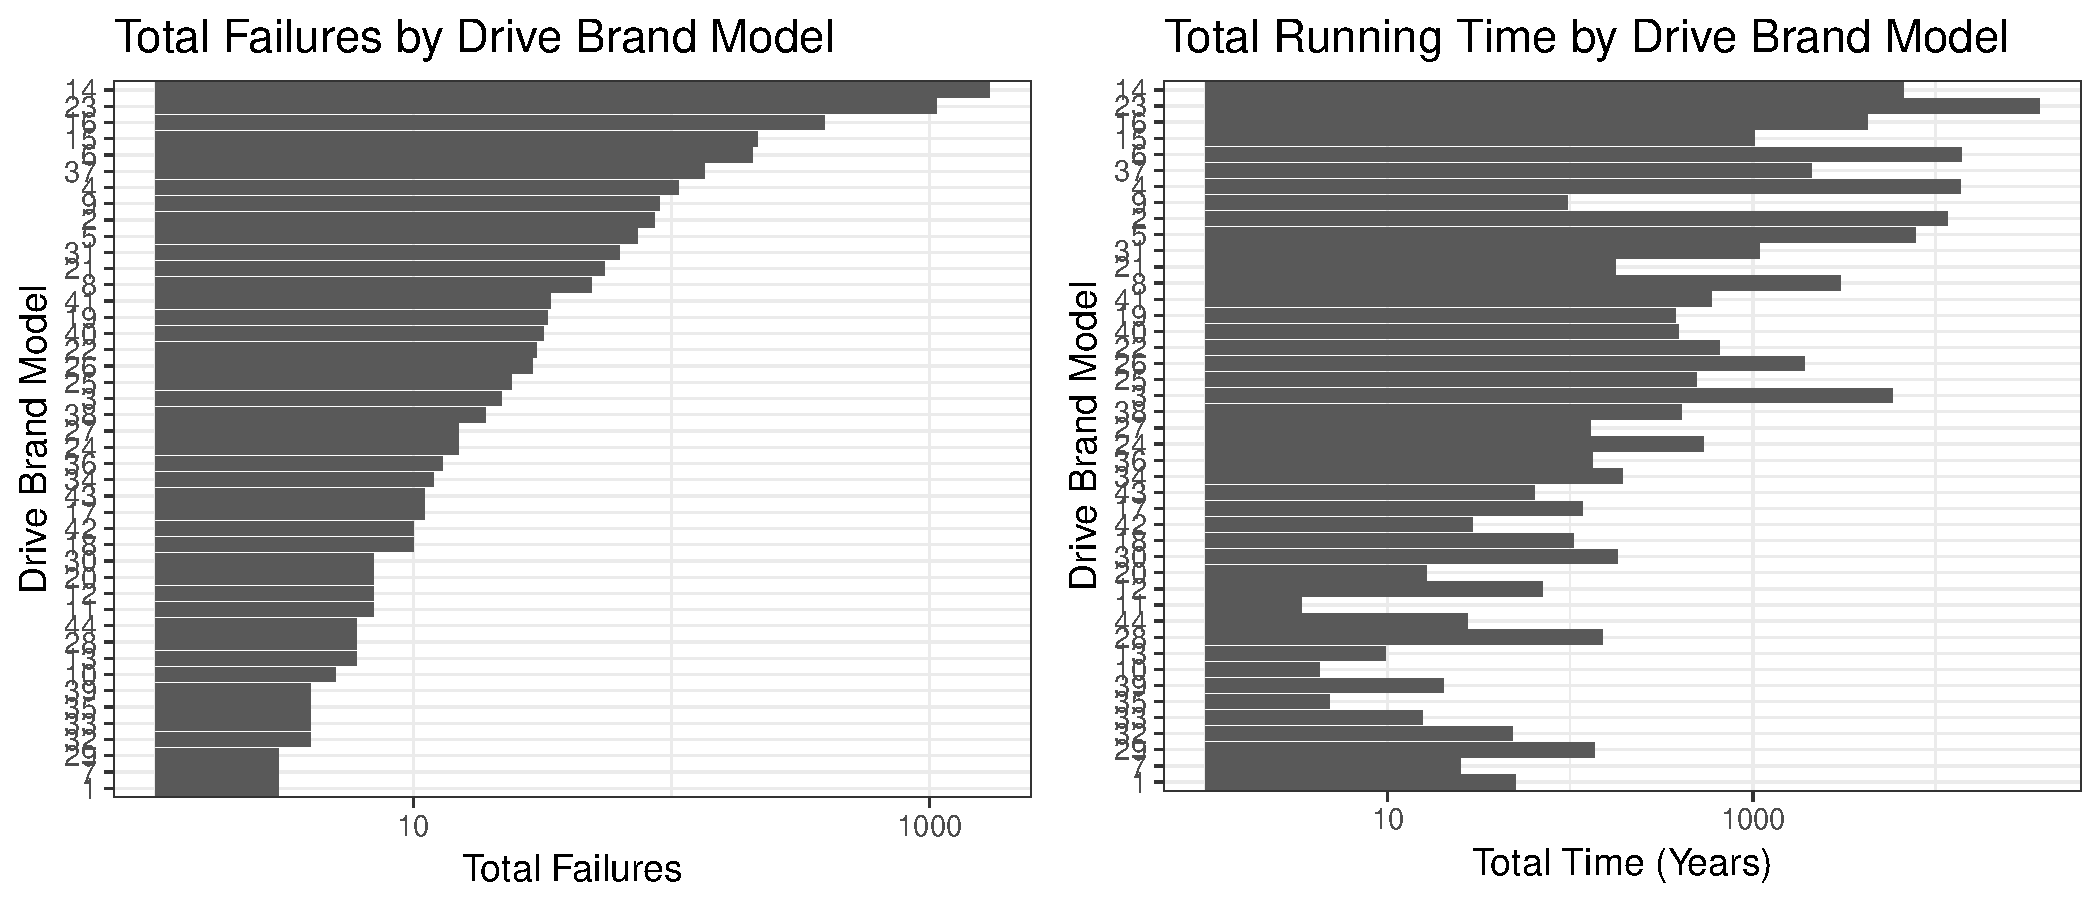
\includegraphics[width=.9\textwidth]{data-sum.pdf}
  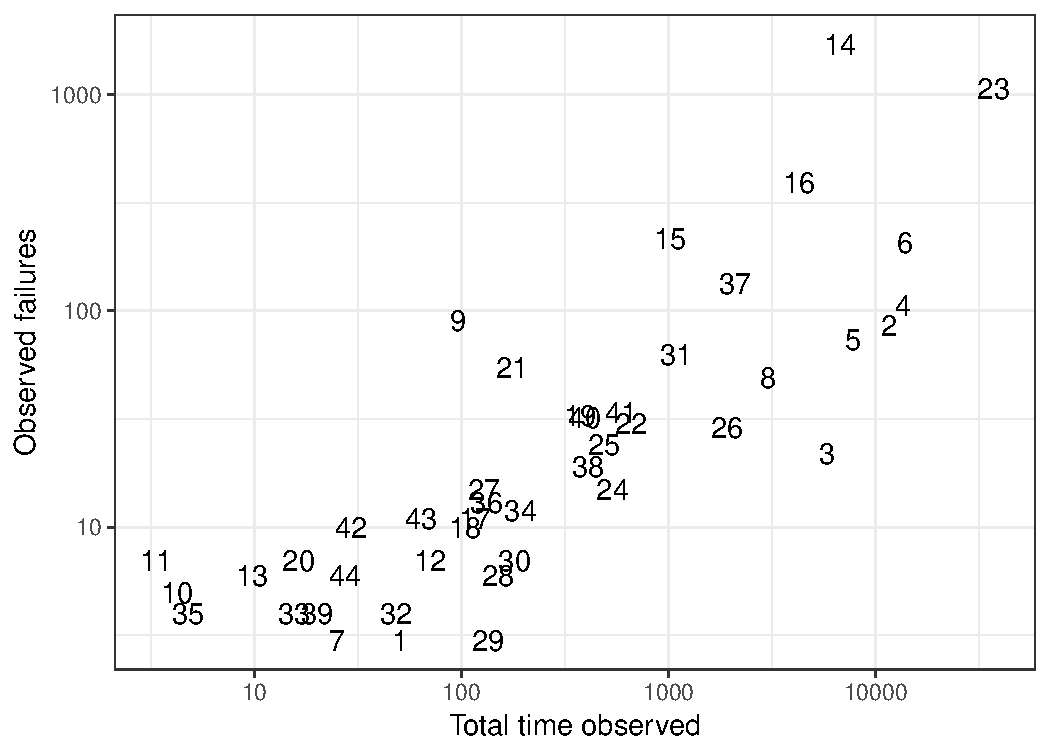
\includegraphics[width=.9\textwidth]{dm-summ-scatter.pdf}
  \caption{Scatterplot of total observed running time (hundred thousands of hours) versus total number of observed failures.  Each number labels a unique drive brand model.   Axes are on the log scale.}
  \label{drive-scatter}
\end{figure}

\subsection{Analysis of a Single Drive-Model}
\label{subsec:ex1}
To illustrate the GLFP model, we will present an analysis of the drive-model with the most observed failures, Drive-model 14.  The Kaplan-Meier estimate plotted below suggests at least two failure modes.  The curve has a slow ramp up in failures till about 10,000 hours (early failures), increases more rapidly from about 10,000 to 20,000 hours (presumably wearout failures).  In addition, computer hard drives are known to have a mixture of early and late failures \citep{chan}.  Therefore, there is both an empirical and theoretical justification to apply the GLFP model.

\begin{figure}[H]
\centering
  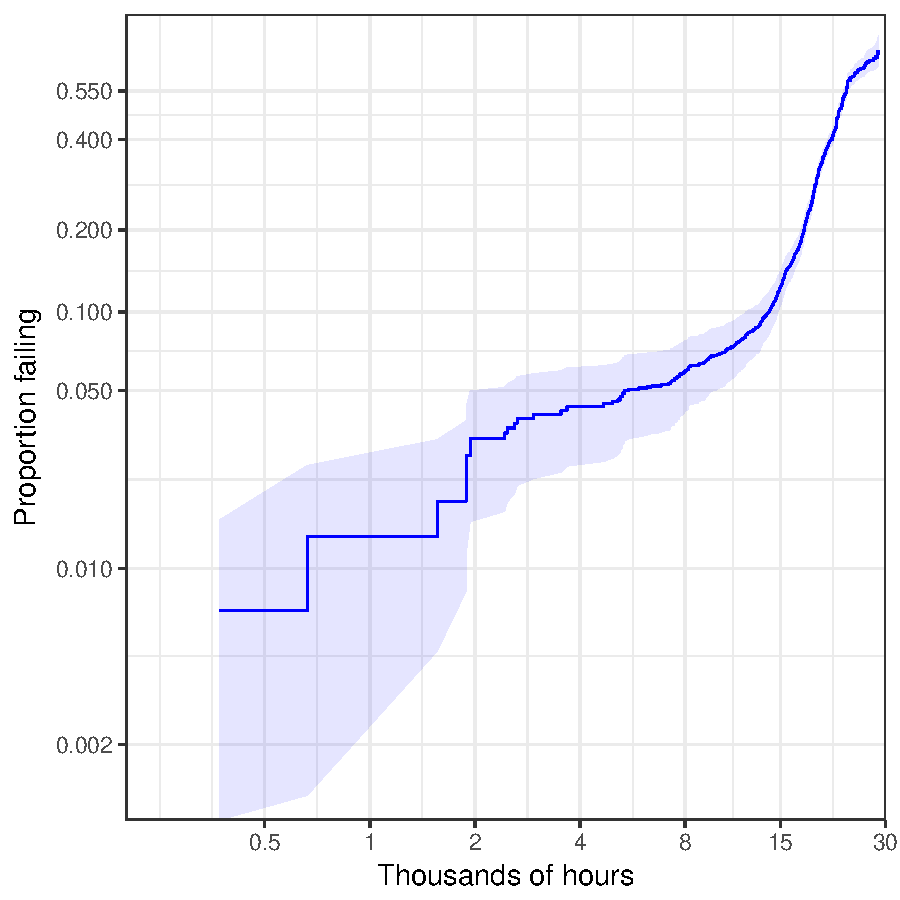
\includegraphics[width=.8\textwidth]{km14-prob}
  \caption{Kaplan Meier estimate for Drive-model 14.  Uncertainty band correspond to pointwise standard errors (using Greenwood's formula.)}
  \label{fig1}
\end{figure}


To estimate the GLFP we use a Bayesian approach, selecting proper prior distributions to improve identification of the model parameters, which also ensures a proper posterior distribution. We reparameterize the component Weibull distributions using the $0.50$ quantile for the infant mortality failure mode ($t_{0.5,1}$) and the $0.20$ quantile for the wearout failure mode ($t_{0.2,2}$). \\

When eliciting prior distribution information it is much easier to ask about recognizable characteristics of a distribution instead of the parameters of the distribution.  Following the approach used in \cite[Section 15.2.2]{intervals} we will use diagonal braces ($\langle.,.\rangle$) to refer to $95$ percent central probability intervals, rather than the standard model parameters when specifying prior distributions.

%$$t_{0.5,1} \sim \op{Lognormal}(8,4), \quad t_{0.2,2} \sim \op{Lognormal}(10,4)$$
$$t_{0.5,1} \sim \op{Lognormal} \langle 1.7,7.6\times 10^6 \rangle,\quad
t_{0.2,2} \sim \op{Lognormal}\langle 8.6, 5.6\times 10^7 \rangle$$
$$\mbox{logit}^{-1}\pi \sim \op{Logitnormal}\langle 1.0\times 10^{-3}, 7.1\times 10^{-1} \rangle,\quad
\sigma_1, \sigma_2 \sim \op{Lognormal}\langle 7.4 \times 10 ^{-3} ,1.3 \times 10^2 \rangle $$
%\quad \sigma_2 \sim \op{Lognormal}\langle 7.4 \times 10 ^{-3} ,1.3 \times 10^2  \rangle $$

These prior distributions put probability mass on a wide range of values for all model parameters, much larger than we would expect for a typical Weibull distribution.  Thus, we consider the priors to be relatively uninformative. 


Table 1 gives the posterior median and 95\% credible intervals for the 5 GLFP parameters for Drive-model 14.  The parameter $p$ is an estimate of the proportion of drives susceptible to to infant mortality.  As expected, this fraction is small with a median value of 0.05.  The parameter $\pi$ estimates for the two Weibull distributions also match intuition.  The infant mortality failure mode puts posterior probability on a values of $\beta_1$ less than 1, which corresponds to a decreasing hazard.  Conversely, the credible interval for $\beta_2$, the wearout mode, is strictly above 1, implying an increasing hazard function.  The two means times to failure (on the log scale) are also well identified with the infant mortality failure mode having an earlier mean time to failure than the wearout mode. 

\begin{table}[H]
\centering
\begin{tabular}{rrrr}
  \hline
 & 2.5\% & 50\% & 97.5\% \\ 
  \hline
$\pi$ & 0.03 & 0.05 & 0.10 \\ 
 $\beta_1$ & 0.47 & 1.13 & 1.72 \\ 
  $\beta_2$ & 4.47 & 4.70 & 4.95 \\ 
  $\mu_1$ & 7.46 & 8.06 & 8.76 \\ 
  $\mu_2$ & 10.12 & 10.13 & 10.14 \\ 
   \hline
\end{tabular}
\caption{Posterior 95\% Credible Intervals for the 5 GLFP parameters for Drive-model 14.}
\label{table:1}
\end{table}

Probability plotting is a simple method to assess the adequacy of (log)location-scale families of probability models to the data.  After properly transforming the axes of a plot, graphing an empirical estimate of fraction failing as a function of time along with simultaneous confidence bands provides a visual check for distributional goodness of fit.  We applied this method using the Kaplan-Meier non-parametric estimate of the empirical cdf.  With left truncation, however, the standard Kaplan-Meier estimator is biased, so we used an adjusted version due to \cite[Chapter 11]{meeker} (see Appendix for a detailed description).   

In Figure \ref{ex1-overlay}, we overlay the posterior median of the fitted GLFP model onto the adjusted Kaplan-Meier estimate with axes on the Weibull probability scale.  Pointwise uncertainty bands associated with each estimator are included. While the Weibull model is inadequate for these data, the GLFP model fits quite well, as it is able to capture the acceleration of the hazard rate between 8000 and 20,000 hours. %The discrepancy around 30,000 suggests that the GLFP may overestimate the proportion failing in the far right tail of the distribution.  While this discrepancy may appear troubling, we suggest that the right tail is of less importance for electronic goods due to obsolescence.

\begin{figure}[H]
\centering
  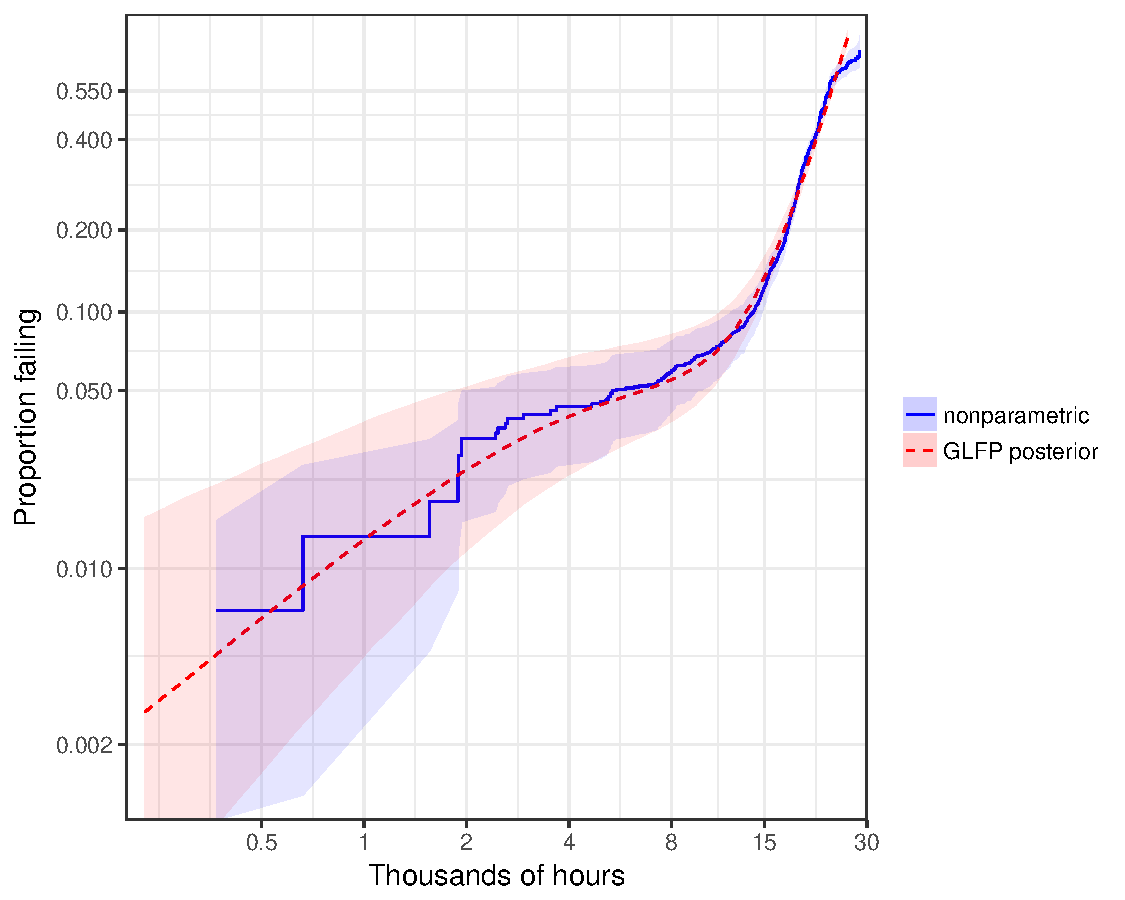
\includegraphics[width=.8\textwidth]{km14-prob-plus}
  \caption{Estimated GLFP for Drive-model 14 plotted on Weibull paper.  Dashed line corresponds to the median of the posterior draws; pointwise 90\% credible band is in red.  Solid line is a non-parametric estimate with pointwise 90\% uncertainty band in blue.}
  \label{ex1-overlay}
\end{figure}


\section{Hierarchical GLFP model}
\label{sec:Hierarchical GLFP model}

In order to describe the entire population, consisting of different but similar sub-populations, and because of the limited amount of data from many of the sub-populations, we model the sub-population specific parameters hierarchically, borrowing strength across the sub-populations.  Let
\begin{equation}
y_{ig} \ind \op{GLFP}\left( \pi_g, \mu_{1g}, \sigma_{1g}, \mu_{2g}, \sigma_{2g} \right),
\end{equation}
where $g=1,\ldots,G$ indexes the sub-populations.  The likelihood for the hierarchical GLFP is a function of $\bm{\theta_g} = (\mu_{1g}, \sigma_{1g}, \mu_{2g}, \sigma_{2g}, \pi_{g})$.  Assuming the lifetimes of all units are independent within and across groups, the likelihood for the data, $i=1,\dots,n_g$,  is given by
\begin{equation*}
L(\bm{\Theta})= \prod_{g=1}^{G} \prod_{i=1}^{n_{g}} \left[\frac{f(t_{ig};\bm{\theta_g})}{1-F(t_{ig}^L;\bm{\theta_g})}\right]^{1-c_{ig}} \left[ \frac{1-F(t_{ig};\bm{\theta_g})}{1-F(t_{ig}^L;\bm{\theta_g})} \right]^{c_{ig}}
\end{equation*}
where $t_{ig}$ is the end of the observed lifetime of unit $i$ in group $g$; $t_{ig}^L$ is the left truncation time for unit $i$ in group $g$; and $c_{ig}$ is an indicator if unit $i$ in group $g$ is right censored.  All times are again in hours.

Next, we model these parameters themselves as random variables, varying across the different sub-populations.  Let
\begin{equation*}
\sigma_{1g} \ind \op{Lognormal} \left( \eta_{\sigma_1}, \tau^2_{\sigma_1} \right)
\end{equation*}
\begin{equation*}
\sigma_{2g} \ind \op{Lognormal} \left( \eta_{\sigma_2}, \tau^2_{\sigma_2}\right)\op{T}\left(0, 1\right)
\end{equation*}
\begin{equation}
\label{eq:hier-model}
t_{p_{1}g} \equiv \mu_{1g} + \sigma_{1g}\,\Phi^{-1}(p_1)  \ind \op{Lognormal} \left(\eta_{t_{p_1}}, \tau^2_{t_{p_1}}\right)
\end{equation}
\begin{equation*}
t_{p_{2}g} \equiv \mu_{2g} + \sigma_{2g}\,\Phi^{-1}(p_2)  \ind \op{Lognormal} \left(\eta_{t_{p_2}}, \tau^2_{t_{p_2}}\right)
\end{equation*}
\begin{equation*}
\op{logit} \pi_g \ind \op{N}(\eta_\pi, \tau_\pi).
\end{equation*}

As discussed in Section \ref{sec:Weibull parameterization}, we reparameterize the Weibull distribution in terms of log quantile and scale since the data we encounter are more informative about the left side of their respective lifetime distribution. We truncate the distribution of $\sigma_{2g}$ at $1$, restricting the wearout failure mode to have an increasing hazard function. We choose to model these parameters (or suitable transformations) with normal distributions because many populations require strong regularization which the normal, with its exponentially decreasing tails, provides. 

In principle, we prefer this full model because we tend to believe that every population has a distribution with a distinct set of parameters. In practice, however, we may consider restrictions to reduce the number of parameters if the data do not support their inclusion. For example, we may consider a model with a common $\sigma_{1}$, letting $\sigma_{1g}=\sigma_1$ for all $g=1,\ldots,G$. A practical strategy is to begin with a simple model and gradually add complexity, reevaluating model adequacy at each iteration. In Section \ref{sec:Model Comparisons}, we illustrate this process, fitting a series of models with increasing complexity and evaluating their performance using a measure of leave-one-out predictive error.


\section{Analysis of the Backblaze hard drive data}
\label{sec:Data analysis}
\subsection{Modeling}
We considered four models, all based on (\ref{eq:hier-model}), which are identified by which model parameters are held constant across drive-models. These are (from most to least restrictive):

\begin{enumerate}
\item $\pi_{g} = \pi,\quad \mu_{1g} = \mu_1,\quad \sigma_{1g}=\sigma_1,\quad \mu_{2g} = \mu_2,\quad \sigma_{2g} = \sigma_2$
\item $\pi_{g} = \pi,\quad \mu_{1g} = \mu_1,\quad \sigma_{1g}=\sigma_1,\quad \sigma_{2g} = \sigma_2$
\item $\pi_{g} = \pi,\quad \mu_{1g} = \mu_1,\quad \sigma_{1g}=\sigma_1$
\item $\mu_{1g} = \mu_1,\quad \sigma_{1g}=\sigma_1$
\end{enumerate}

The set of model specifications were chosen based data, interpretation of the model, as well as estimation considerations.  Product specific parameters for the the wearout failure mode $(\mu_{2g},\sigma_{2g})$, and the proportion defective $(\pi_g)$, are considered as a means to account for heterogeneity across brands in the right tails of the failure distribution.  Going from a common model for all product brands and gradually increasing the complexity of the model, we end up at Model 4.  Model 4 allows for the probability of infant mortality as well as the shape and scale parameters for the wearout failure mode to vary by Drive-model.

For all of the models we consider, the parameters for the infant mortality failure mode are held in common across Drive-models.  We found that there was often insufficient information to model these parameters hierarchically.  Moreover, assuming a common distribution for infant mortality provides a meaningful interpretation and comparison of $\pi_g$ and $\pi_{g'}$ ($g \neq g'$). 

\subsubsection{Prior Distributions}
\label{sec:Prior Distributions}
To complete the full probability model, we need to select prior distributions for the parameters governing the hierarchical model. We select proper prior distributions to ensure a proper posterior distributions.

For Models 1-4, different sets of restrictions required different prior distribution specifications, which were assigned as follows:

\paragraph{Model 1.} Constrain all Drive-models to the same GLFP distribution. For this ``reduced" model we assume the same prior distributions as in Example 1.

\paragraph{Model 2.} $t_{p,g}$ varies by Drive-model. To help with model identifiably, we tighten the priors on the infant mortality failure mode:
$$ \pi \sim \op{Logit-normal}\langle 7.0\times 10^{-3},\, 2.6 \times 10^{-1} \rangle,$$
$$\sigma_1 \sim \op{Log-normal}\langle 1.4 \times 10^{-1},\, 7.1\rangle,$$ 
$$t_{p1} \sim \op{Log-normal} \langle 2.2 \times 10^1,\, 5.5 \times 10^{4} \rangle.$$

\paragraph{Model 3.} $t_{p,g}$ and $\sigma_{g2}$ vary by drive-model. Priors for constrained parameters are the same as for Model 2.

\paragraph{Model 4.} $\pi_g$, $t_{p,g}$ and $\sigma_{g2}$ vary by drive-model. Priors for constrained parameters are the same as for Model 2.


Where applicable prior distributions on hyperparameters are as listed below. We follow the recommendation of \citet{gelman2014bayesian} to use half-Cauchy prior distributions on hierarchical scale parameters. As for the location hyperparameters, we choose weakly informative prior distributions centered around the corresponding prior mean for the non-hierarchical model.
% The prior for $\eta_\pi$ puts 95\% of prior mass on the interval $(0.006, 0.27)$ for the median proportion defective (What justification? Should maybe be lower.) For $\eta_{\sigma, 2}$, $95\%$ of prior mass is on values greater than $0.037$. Since $\sigma_d$ is the reciprocal of the Weibull shape parameter, this corresponds roughly to an assumption that the median Weibull shape parameter is less than $1/0.037 = 27$. The prior for $\eta_{t_{p_2},2}$ implies that the median 20th percentile for non-defective units is less than greater than 3 days and less than 24 years.

\begin{align*}
  \eta_{\pi} & \sim \op{Normal}(-3, 1)\\
  \tau_{\pi} & \sim \op{Half-Cauchy}(0, 1)\\
  \eta_{\sigma ,2} & \sim \op{Normal}(0, 2)\\
  \tau_{\sigma ,2} & \sim \op{Half-Cauchy}(0, 1)\\
  \eta_{t_{.2_2},2} & \sim \op{Normal}(9, 2)\\
  \tau_{t_{.2_2},2} & \sim \op{Half-Cauchy}(0, 1).
 \end{align*} 

\subsection{Computation}
\label{sec:Computation}
Each model was fit using the {\tt
  rstan} \citep{rstan} package in {\tt R} \citep{r}, which implements a variant of Hamiltonian Monte Carlo (HMC)
\citep{betancourt}. HMC jointly updates all model parameters by simulating energy preserving paths with random initial momentums along the posterior density. This is done to reduce autocorrelation and efficiently explore the posterior. Multiple chains were run for 1500 iterations after 1500 warmup iterations: 4 chains were run for Models 1, 2 and 3 and 16 chains were run for Model 4. The Gelman-Rubin potential scale reduction factor was used to provide a check for adequate mixing of the multiple chains. Upon convergence, $\hat{R}$, converges to 1.  The  maximum values of $\hat{R}$ across all model parameters for Models 1 throught 4 (5, 50, 95 and 140 parameters, respectively) were 1.005, 1.028, 1.009 and 1.004. Other diagnostics provided by the software (tree-depth, and divergent transitions) were clean. Plots of the posterior draws were inspected for parameters with the fewest effective samples; these did not suggest features that were inadequately explored.

% HMC generates proposals by simulating paths along the posterior density. This is done to reduce autocorrelation between samples, but doing so also provides a useful diagnostic. \textit{Divergent transitions} will tend to occur when the posterior has regions of high curvature, which can present problems for MCMC by making it difficult to fully explore the posterior distribution. This feedback can be useful 



\subsection{Model Selection}
\label{sec:Model Comparisons}
As we have discussed, while we prefer to allow all of the GLFP model parameters to be Drive-model specific, there are practical issues with fitting the full model. For example, due to heavy left-truncation, there may be insufficient information for particular Drive-models to estimate all of the parameters. 

Figure \ref{fig:fig2} provides a visual comparison for Models 1 through 4 by plotting the pointwise posterior median of time to failure. The large left panel shows the Kaplan-Meier nonparametric estimate of the same. The Kaplan-Meier estimates on the right side of Figure \ref{fig:fig2} shows that the set of estimated failure curves for all four models that we fit. The smaller plots correspond to Models 1 through 4 reading from left to right, top to bottom. Note that while all the paths for the posterior estimates necessarily pass through the origin, the nonparametric curves do not, but only because, for the Kaplan-Meier estimator, inference is entirely conditional on survival up to left-most left-trunctation time; to make the plot comparable, we use an adjustment based on a parametric model (Model 4).

%Should we be brief discussing the plot?
These plots suggest that Model 1 is insufficient to explain the observed data. Model 2 certainly captures more of the heterogeneity observed in the Kaplan-Meier estimates; we observe that the assumption of a common $\sigma_2(=\sigma_{2,g})$ results in a very similar progressions in the rate of failure, which may be too restrictive. Model 3, which removes this restriction on $\sigma_{2,g}$ suggests that there is evidence to support variation in this parameter among drive-models. While Model 3 and 4 do display differences, their impact is relatively subtle.

\begin{figure}[H]
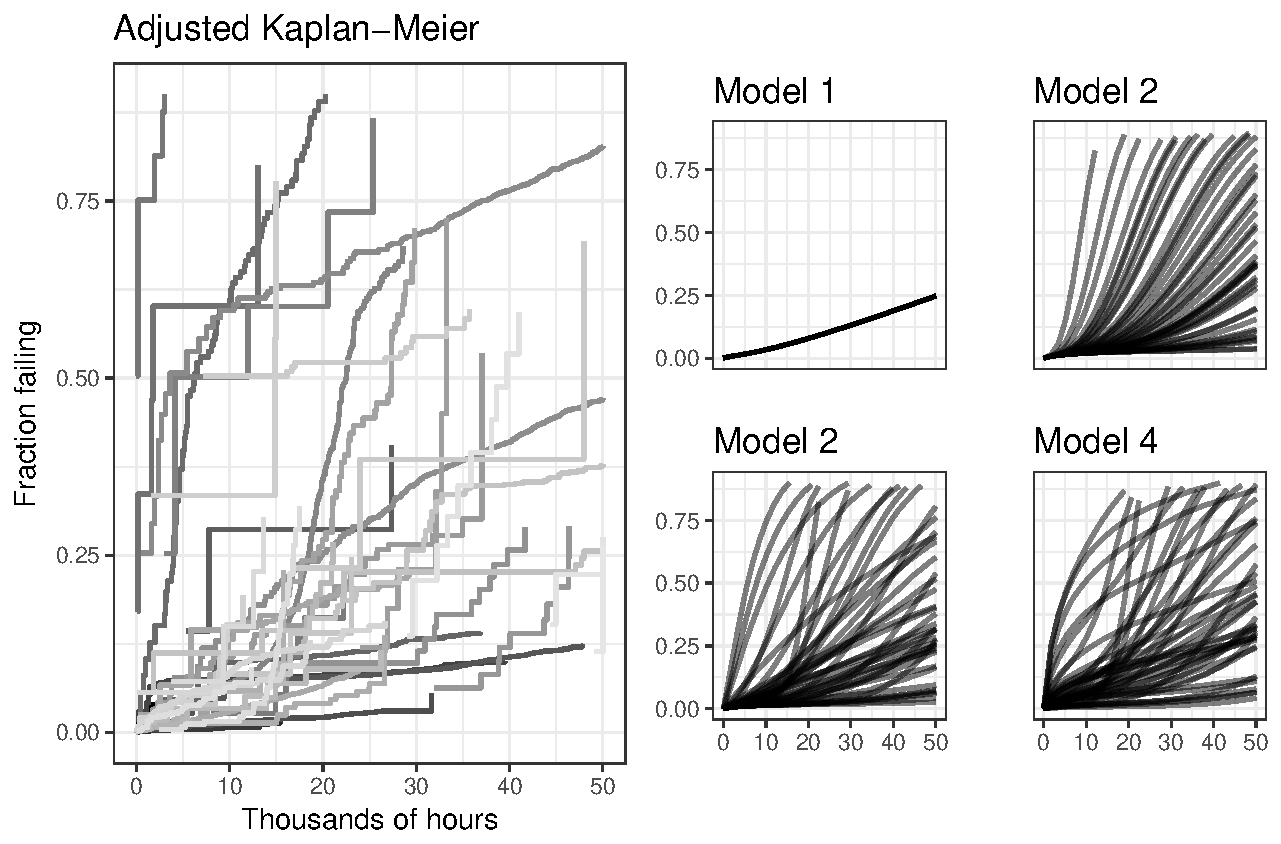
\includegraphics[width=\textwidth]{heterogeneity-compare}
\caption{Left: Kaplan-Meier estimates of the time to failure for each of the Drive-models in the Backblaze data. Right: Pointwise posterior median time to failure curves for Models 1-4, ordered left to right, top to bottom.}
\label{fig:fig2}
\end{figure}

We can also compare the four Model fits for each Drive-model individually.  For these comparisons, we use the posterior median of the MCMC draws. %Unlike maximum likelihood, by including the hyperparameters in the probability model, there is a data-dependent penalization that results in shrinkage toward a common overall model.

\begin{figure}[H]
{\centering
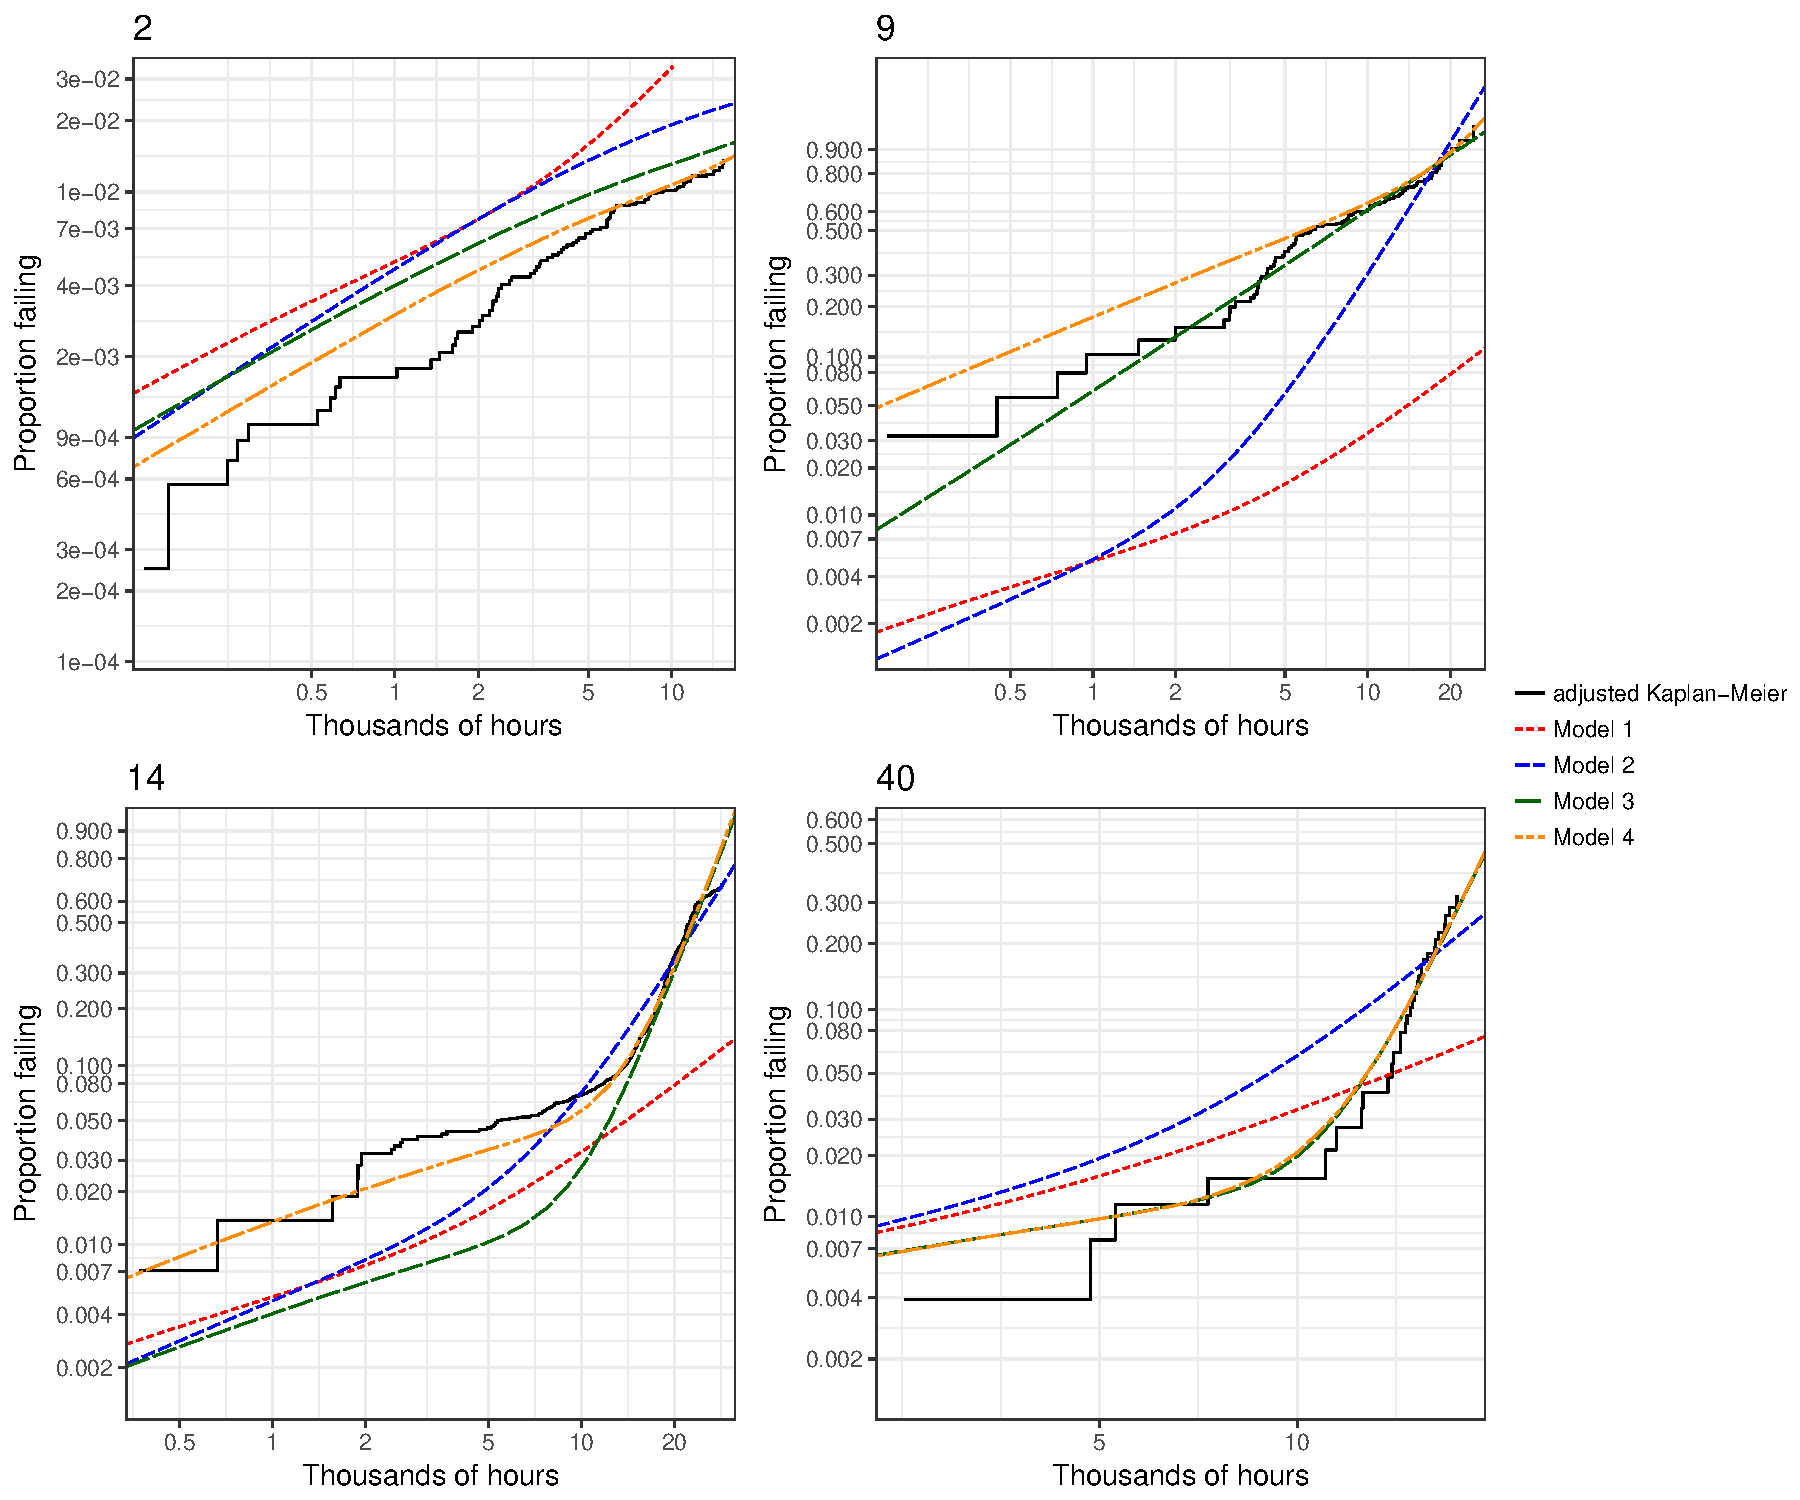
\includegraphics[width=\textwidth]{single-drive-4-Models-ex}}
\caption{Posterior median of proportion failing as a function of time under Models 1-4 for sample of Drive-models, with axes scales as for Weibull probability plotting.  The solid step function is the truncated adjusted Kaplan-Meier points.}
\label{fig:mod_comp_leg}
\end{figure}

The GLFP fit for a representative selection of Drive-models (Drive-models 2, 9, 14, and 40) are presented in Figure \ref{fig:mod_comp_leg} (See the Supplementary Material for all plots).  The black step functions again correspond to the adjusted Kaplan-Meier estimates.  As model complexity increases, the GLFP curves become more flexible and are better able to fit the observed failure data.  All of the GLFP models appear to produce lower estimates, relative to Kaplan-Meier, of the proportion of failed hard drives for Drive-model 2, with Model 4 being in closest agreement.  For Drive-model 14, Models 1-3 produce lower estimates of the proportion of drives failing, and for Drive-model 40, they produce higher estimates.  On the other hand, Model 4 follows the nonparametric estimate quite closely across stages of lifetime.  The differences between Models 3 and 4 and Models 1 and 2 are visually quite apparent.  Differentiating between Model 3 and 4 is less clear; for instance, the estimates from Model 3 and 4 are nearly identical for Drive-model 40.



From the point of view of a consumer of hard disk drives, the goal of an analysis such as this is may be to rate manufacturers and/or to inform future purchases based on predicted product performance. In this case, we should choose the model that will provide the most accurate prediction for future units of previously observed Drive-models. One appropriate criterion for model selection, then, is log pointwise predictive density (lpd),

\begin{equation}
\mbox{lpd} = \sum_{g=1}^G \sum_{i=1}^{n_g} \log[p(t_{new,g,i}|t, t^L, c)] = \sum_{g=1}^G \sum_{i=1}^{n_g} \log \left[ \int p(t_{new,g, i}|\theta) p(\theta|t,t^L,c) d\theta \right].
\end{equation}

Using this criterion, we should choose the Model with the highest expected lpd (elpd) for a new data set $\{t_{new,g,i}:g=1,\ldots,G; i=1,\ldots,n_g\}$. Suppressing the conditioning on $t^L$ and $c$,
\begin{equation}
\mbox{elpd} = \op{E}_h \mbox{lpd} = \sum_{g=1}^G \sum_{i=1}^{n_g} \int \log [p(t_{new, g, i}|t)] h(t_{new,g,i}) d t_{new,g,i},
\label{elpd}
\end{equation}
where $h$ is a density for the true distribution of $t_{new,g,i}$. Although $h$ is unknown, leave-one-out cross-validation provides a robust estimator:
\begin{equation}
\widehat{\text{elpd}} = \sum_{g=1}^G \sum_{i=1}^{n_g} \log [p(t_{g,i}|t_{-(g,i)})].
\label{loo-est}
\end{equation}
The \texttt{R} package, \texttt{loo} \citep{loo}, computes an approximation of (\ref{loo-est}) provided that the observations $t_i$ are conditionally independent. It employs an importance sampling method that uses $S$ saved MCMC draws to compute smoothed importance weights, $w_{i,s}$, approximating $\log [p(t_{g,i}|t_{-(g,i)})]$ with $\frac{\sum_{i=1}^S w_{i,s} p(t_{g,i})}{\sum_{s=1}^S w_{i,s}}$. In addition to providing an estimate of (\ref{elpd}), their method also produces a standard error based on an asymptotic result. For details, refer to \cite{vehtari}.
%When $n$ is large, the distribution of the elpd is approximately normal and different models can be compared statistically. 
% To statistically compare the GLFP Models, we estimated the predictive accuracy of the 4 different models using an approximate leave-one-out cross validation (LOO) method.  As outlined in Vehtari et. al, the predictive accuracy from a fitted Bayesian model can be estimated simply with posterior draws of the model parameters rather than re-fitting the model with different data sets \cite{vehtari}.  For each observation, $i$, the log point-wise predictive density is calculated over the full set of posterior samples with data point $i$ removed.  
% The final expected log point-wise predictive density (elpd) is the sum over all observations (elpd $=\sum{\log p(y_i|y_{-i})}$).  
Results showing estimated elpd and associated standard errors for all 4 models are shown in Table \ref{table:2}.
 We calculated the difference in expected predictive accuracy for Model 4 versus 3, Model 3 versus 2, and Model 2 versus 1, as well as the standard error of the difference (Table 1).  
For the models we considered, each successive increase in model complexity increases elpd.  Of all the models, Model 4 has significantly better elpd compared to the the other 3 models.
\begin{figure}
\begin{table}[H]
\centering
\begin{tabular}{rrrrrrr}
  \hline
 & $\widehat{\text{elpd}}$ \ & Difference in $\widehat{\text{elpd}}$ \ & SE of the Difference \\ 
  \hline
Model 4 & -13309.5 & 40.7 & 11.3 \\ 
Model 3 & -13350.2 & 458.8 & 31.0  \\ 
Model 2 & -13809.0 & 3674.6 & 96.2 \\ 
Model 1 & -17483.6  \\ 
   \hline
\end{tabular}
\caption{Expected Log Pointwise Predictive Density (elpd) for each model specification.  Each model is compared to the more parsimonious model below.  The estimated difference of expected leave-one-out prediction errors between the two models, as well as the standard error of the difference, is also presented.}
\label{table:2}
\end{table}
\end{figure}
\subsection{Results}
\subsubsection{Model Assessment}
Having chosen Model 4 as the best of the candidate models, we would like to assess whether our model provides an adequate fit to the observed data. One way to do this is to draw replicate data sets from the posterior predictive distribution. This is a general approach recommended by \cite{gelman1996postpred} for models where no classical goodness-of-fit test is available. In the hierarchical setting, there can be different formulations of the predictive distribution. In the present context, one could predict the lifetime of a new unit of a previously observed Drive-model or a new Drive-model. We choose to focus on the former.  There are many possible approaches to the posterior predictive check. For this problem, we chose to consider the posterior predictive distribution of the Kaplan-Meier estimate for each Drive-model $g$.

% Graphical comparisons can be highly informative in revealing limitations of the model. as in our cas a graphical posterior predictive check, wherein replicate data sets are generated from the posterior predictive distribution and compared with the observed data. Because of the rich information gleaned from plotting the data, this method can be very effective at identifying limitations of the model.


Because the variability in the Kaplan-Meier is primarily a function of the number of at-risk units, we want to replicate the pattern of censoring that was observed. That is, for unit $i$ of drive-model $g$,
$$p(t_{rep,g}) = \int \prod_{i=1}^{n_g}f(t_{new}|t_{g,i}^L,c_{g,i},\theta)\,p(\theta|t)d\theta.$$
Because we are working with posterior draws, $\theta^{(s)}$, we can draw from this distribution by choosing $\theta^{(s)}$ at random, then conditionally draw $t_{rep,g}$ from $f(t_{new}|t_{g,i}^L,c_{g,i},\theta^{(s)}).$

An obstacle remains, in that the censoring mechanism itself is not fully observed. Our admittedly simple approach is to assume that failed units would have been the censored had they survived until the latest censoring or failure time for that drive model. We chose to generate 19 replicates for each drive model. This gives a 1/20 chance under the hypothesis of no difference that the Kaplan-Meier estimate based on the observed data would be ``most extreme" relative all the replicated  from the those one and is not too many so as to produce an overly cluttered plot. Our method for generating replicate data sets, $y_{rep,g}^{(s)}$, $s = 1 \dots 19$, for each Drive-model $g=1,\ldots,44$, is as follows:
\begin{enumerate}
\item Simulate $\tilde{t}_{rep,g,i}^{(s)} \sim \op{GLFP}(\pi_{g}^{(s)},\mu_1^{(s)},\sigma_1^{(s)},\mu_{2g}^{(s)}, \sigma_{2g}^{(s)})$ where each set of parameters, $\left( \pi_{g}^{(s)},\mu_1^{(s)},\sigma_1^{(s)},\mu_{2g}^{(s)}, \sigma_{2g}^{(s)} \right) $, is a random draw from the full posterior distribution.
\item Repeat step 1 until $\tilde{t}_{rep,g,i} > t_{g,i}^L$.
\item If $c_{g,i}=0$, let $c_{rep,g,i}^{(s)}=\max \{t_{g,i}: i \ge 1\}$, otherwise let $c_{rep,g,i}^{(s)}=t_{g,i}$.\\
If $\tilde{t}_{rep,g,i}^{(s)}>m_{g,i}$, set $t_{rep,g,i}^{(s)}=c_{rep,g,i}^{(s)},\; c_{rep,g,i}^{(s)}=1$, otherwise set $t_{rep,g,i}^{(s)}=\tilde{t}_{rep,g,i}^{(s)},\; c_{rep,g,i}^{(s)}=0$.
\end{enumerate}

\begin{figure}[H]
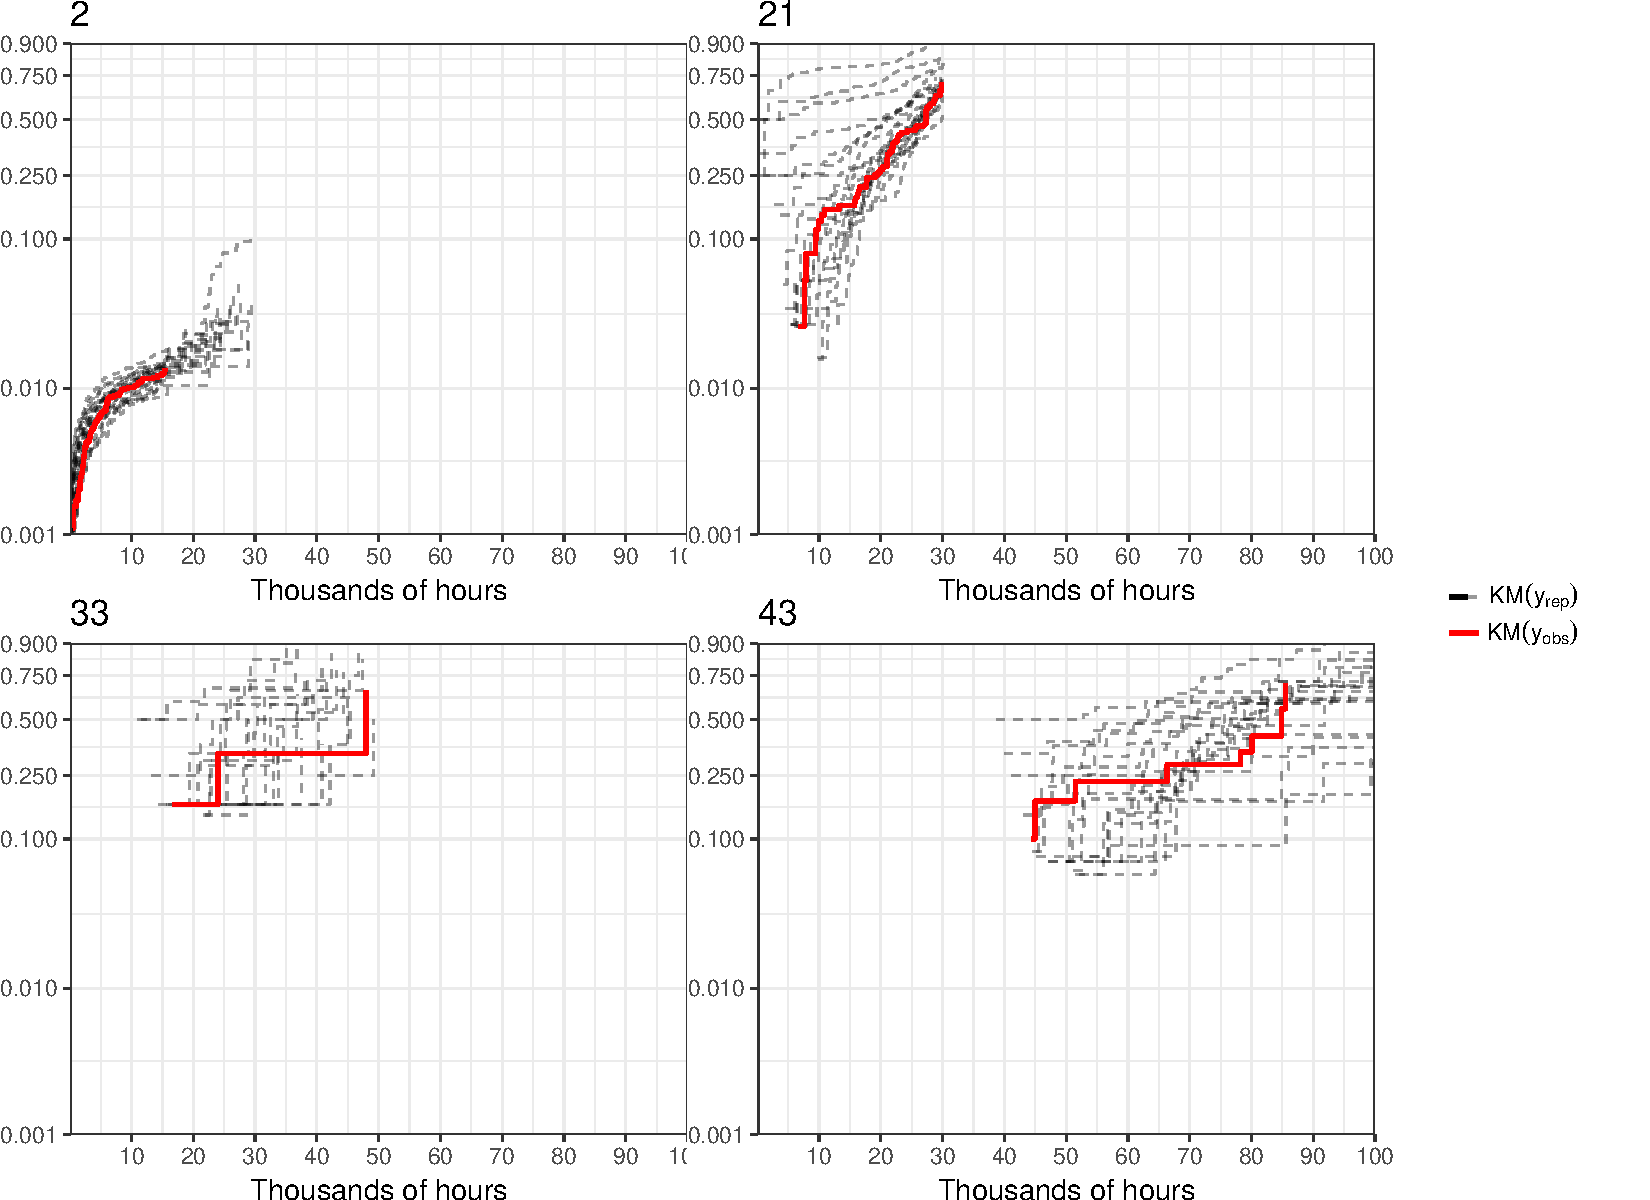
\includegraphics[width=\textwidth]{ppcheck-sample}
\caption{Nonparametric estimates of proportion failing for a representative subset of Drive-models. Both the original data (\textbf{bold} line) and 19 ``replicated" data sets from the posterior predictive distribution (\textit{dashed} lines) are shown.}
\label{fig:post-pred-KM}
\end{figure}

We can compare the 19 simulated data sets $y_{rep,g, i}$ to the observed data $y_{g,i}$ by using them to re-estimate the Kaplan-Meier nonparametric estimator. The resulting plots are displayed in Figure \ref{fig:post-pred-KM}. Only a representative sample of plots are shown here for brevity (see the Supplementary Material for the complete set of Drive-models).  For most Drive-models, the estimates based on the observed data look similar to those based on the replicated data.  There are a few Drive-models, however where this is not the case. As we addressed previously, in Subsection \ref{subsec:ex1}, Drive-model 14 has a discrepancy between the GFLP and the Kaplan-Meier fits in the right tail. Due to the large number of failures for this Drive-model, the posterior for the hierarchical model is very similar to the stand-alone model, so all the same comments made earlier still apply. In addition, Drive-models 4, 11 and 34 appear to be exceptions as well. We will focus our attention on Drive-model 4, but our diagnosis of 34 is similar, so the following comments extend to that Drive-model as well.


To attempt to diagnose the cause of the discrepancies between the observed data for Drive-model 4 and its posterior predictive distribution, we plot an event plot for a random sample of units for this Drive-model, along with the Kaplan-Meier estimate, and the posterior estimate of time to failure (see Figure \ref{fig:ex-mod-4}). From these plots, it appears that the large discrepancy between the posterior and the nonparametric estimate is driven by a small number of failures that occur in the several thousand hours, at a time where very few units were observed to be at risk. In further support of this hypothesis, if we ignore records with observation periods that include the first quarter, the modified nonparametric estimate falls within the posterior 90\% pointwise credible band. While it might be tempting to treat those early failures as anomalous, they also point to a weakness in our model. By virtue of having all Drive-models share in common the Weibull parameters for the infant mortality failure mode, an early rash of failures indicating a subpopulation with, say, an increasing hazard function,  would be problematic. While the proportion at risk of early failure can vary via $\pi_g$, the plausible values of the common parameters, $\mu_1$ and $\sigma_1$, do not ``line up" in a way so to influence the posterior as they might have had they been allowed to vary. In other words, the problem seems to go away much quicker than would be expected under Model 4.

As another example, to further appreciate how information is being borrowed across groups, consider Drive-model 43 (Figure \ref{fig:ex-mod-43}). The data for this Drive-model are heavily truncated; the observed units had run for quite some time before data were made available. In Figure \ref{fig:ex-mod-43} we see that the lack of data for this Drive-model at early ages results in a diffuse posterior centered around the what we call the ``global estimate," corresponding to $\op{GFLP}(\eta_{\pi}, \mu_1,\sigma_1, \eta_{t_2} - \eta_{\sigma_2}\Phi^{-1}(.2), \eta_{\sigma_2})$. Then, in the period where records exist for this Drive-model, at around 10,000 hours, the posterior deviates from the global model, achieving a compromise between it and the nonparametric estimate.



\begin{figure}
\centering
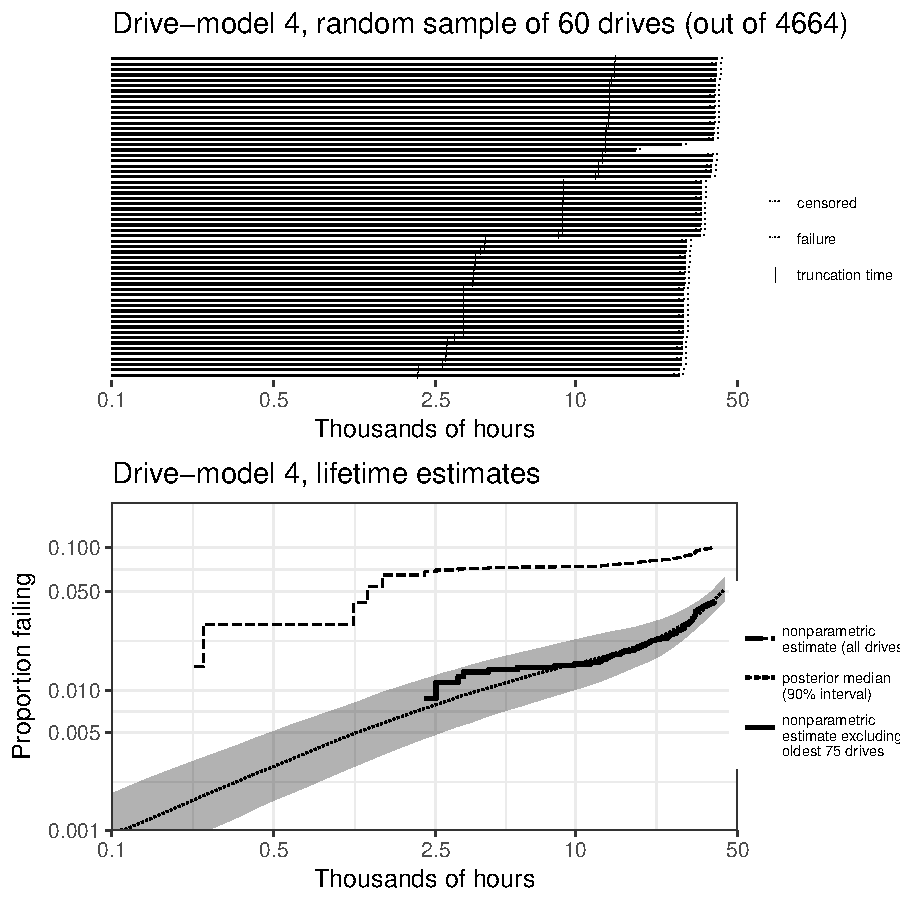
\includegraphics{dm4-exception}
\caption{\small Top: Event plot for uniform random sample of 60 units of Drive-model 4. Left endpoints are left-truncation times, dashed lines extending to the right indicate censoring intervals, $[t_4,i, \infty)$, and right endpoints without joined dashed lines are observed failure times, i.e. $t_{4,i}\mbox{, where }c_{4,i}=0$.\hspace{\textwidth}Bottom: The adjusted Kaplan-Meier estimate (solid step function) substantially higher than the pointwise posterior median (dashed line; shaded region showing 90\% credible interval) due to several early failures while few were at risk.  Using the same Kaplan-Meier estimator, but only the data truncated after 2500 hours (dotted line) shows close agreement with the posterior median.}

\label{fig:ex-mod-4}
\end{figure}

\begin{figure}
\centering
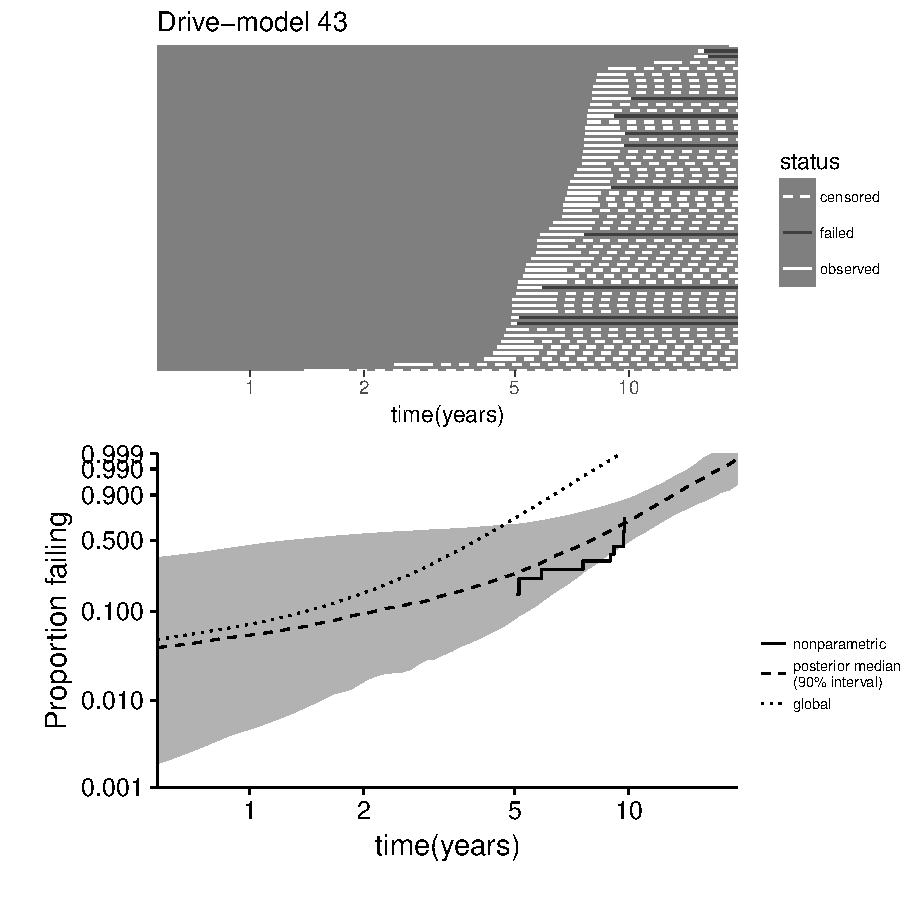
\includegraphics{dm43-shrinkage}
\caption{\small Top: Event plot for all units of Drive-model 43. Left endpoints are left-truncation times, dashed lines extending to the right indicate censoring intervals, $[t_{43},i, \infty)$, and right endpoints without joined dashed lines are observed failure times, i.e. $t_{43,i}\mbox{, where }c_{43,i}=0$.\hspace{\textwidth}Bottom: The solid step function correponds to the adjusted Kaplan-Meier estimate. Due to the absence of collected information about early life for this particular model, due to left-truncation, the posterior median (dashed line) follows the ``global model" (dotted line), i.e. the posterior median of proportion failing for a new Drive-model, approximately until the beginning of the earliest observational period.}
\label{fig:ex-mod-43}
\end{figure}

\subsubsection{Drive-model Comparisons}
\label{subsubsec:Drive-model Comparisons}
We consider the problem of ranking Drive-models. From a
business perspective, it is clear
that we should prefer the Drive-models which will provide more years
of service. For ease of exposition, we will assume that the purchase
price of a hard-drive is the same across Drive-models.

There are two sources of variation at play; the
posterior uncertainty in the parameters, which largely depends on the
sample size, and the uncertainty in future
observations conditional on the parameters. The {\em posterior
  predictive} distribution incorporates both sources.
\begin{equation*}
  p(t_{d,new}|t) = \int p(t_{d,new}|\theta_d) p(\theta_d|t_d) \, d\theta_d
\end{equation*}

We can sample from this distribution by drawing $t_{d,new}^{(s)}$ from
$\operatorname{GLFP}(\pi_d^{(s)},
\mu_1^{(s)},\sigma_1^{(s)},\mu_{2,d}^{(s)},\sigma_{2,d}^{(s)})$, for
$s=1,...,S$, using the saved posterior draws for the model
parameters. The mean time-to-failure (MTTF) for drive-model $d$ can be estimated by
$$\frac{1}{S} \sum_{s=1}^{S} t_{d,new}^{(s)}.$$

While MTTF is clearly important, due to the
anticipation of advancements in technology, we can expect that the
relative value of computer hardware will depreciate rather quickly. In simple terms, given two hard drives, one would prefer to have both of them work for five years than for one to work for ten years and the other to not work at all. To account
for depreciation, rather than using MTTF as the metric for Drive-model comparison, we use the value at replacement. The US Internal Revenue Service considers
computer hardware to be ``5-year'' equipment \citep{f4562}. Using``the declining
balance method'' the rate of depreciation is 40\% per year.

Let $L(t) = e^{-0.4t}$ represent the value at the time of failure
relative to a new unit. We can rank the Drive-models by 
$$\op{E}(L(t_{d,new})|t))\approx \frac{1}{S} \sum_{s=1}^{S} L(t_{d,new}^{(s)}).$$

Posterior credible intervals for $L(t_{d,new})$ are shown in the left panel of Figure \ref{fig5}. A zoomed version of the top 8 Drive-models, as ranked by $\op{E}(L(t_{d,new})|y)$ are shown in the bottom right panel. The panel above shows credible intervals for MTTF. We can see that ranking by MTTF would lead to a different result -- a new Drive-model 8 unit expected to have the last the longest, but possibility of it failing early is higher than for the Drive-models ranked highest by our depreciation-aware metric. The top four Drive-models (4, 5, 2, 3) seem comparable, with a new Drive-model 4 unit expected to depreciate the most. However, given the discrepancy of the model fit for Drive-model 4, noted in the previous subsection, in the absence of more early life data, we might harbor some lingering concern about possible quality-control issues with this Drive-model.

We can also use the posterior draws to compute quantiles of interest, which in reliability applications is typically more informative than a measure of central tendency.  The left panel of Figure 5 shows $t_{0.10}$ (i.e., the amount of time it takes for 10\% of hard drives to fail), for all Drive-models. The best six Drive-models ranked by MTTF are also the Drive-models with the largest $t_{0.10}$.  Drive-models 5, 2, 4, and 3 seem to really stand out as the most reliable as there is a larger gap separating them from the rest of the group.  Another interesting feature to compare is $\pi$, the proportion defective.  The right panel of Figure 5 shows the posterior credible intervals of $\pi$ for each Drive-model.  The plot is again sorted according to $t_{0.10}$ so it can be compared to the left hand side.  While for many of the Drive-models the ordinal ranking is the same as on the left, there are some Drive-model comparisons, for example 23 and 18, that differ in ranking if compared using $t_{0.10}$ or $\pi$.  Depending on a user's application or the hard drive warranty length, using the $\pi$'s as a comparison tool may be a relevant parameter of interest.  

\begin{figure}[H]
\centering
   \begin{subfigure}[b]{0.80\textwidth}
   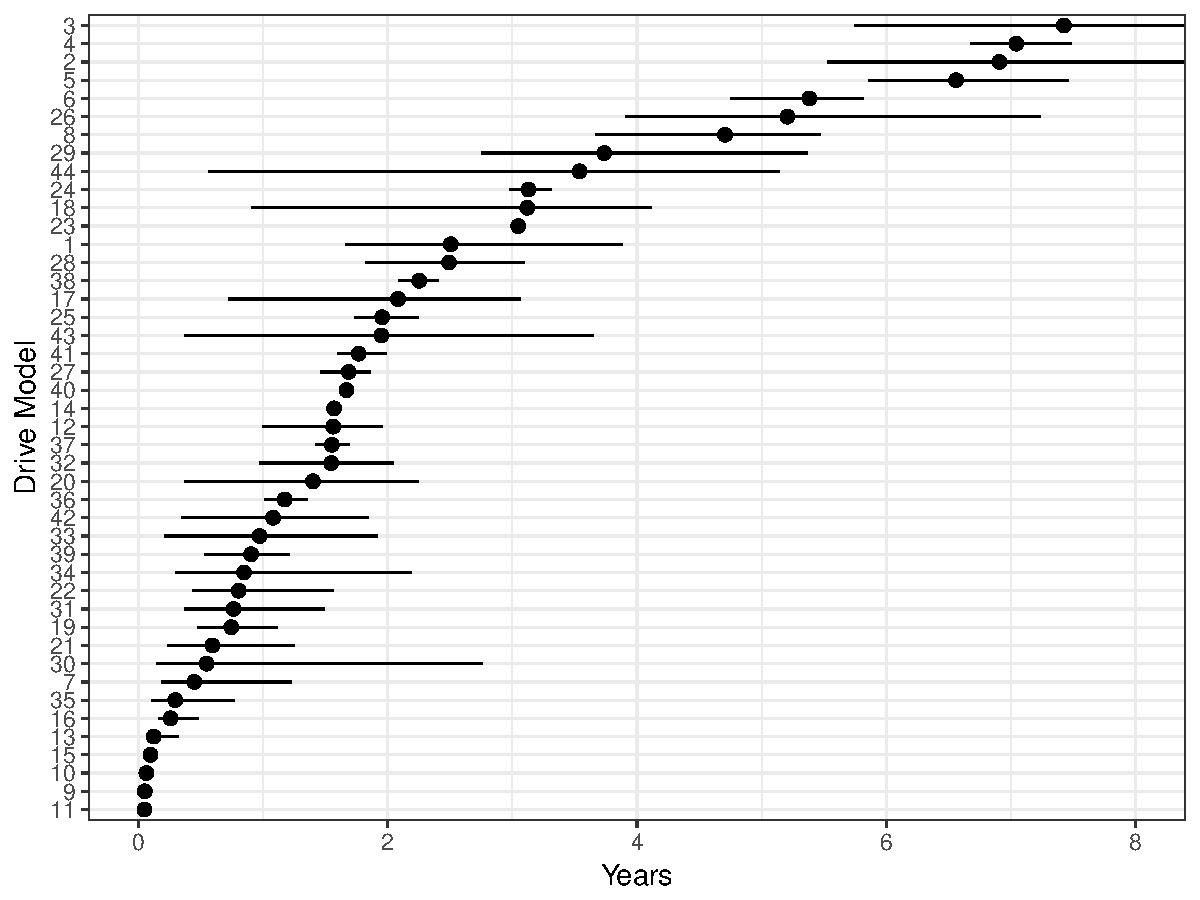
\includegraphics[width=1\linewidth]{b10new.pdf}
   \caption{50\% CI for $t_{0.10}$}
   \label{fig:Ng1} 
\end{subfigure}

\begin{subfigure}[b]{0.80\textwidth}
   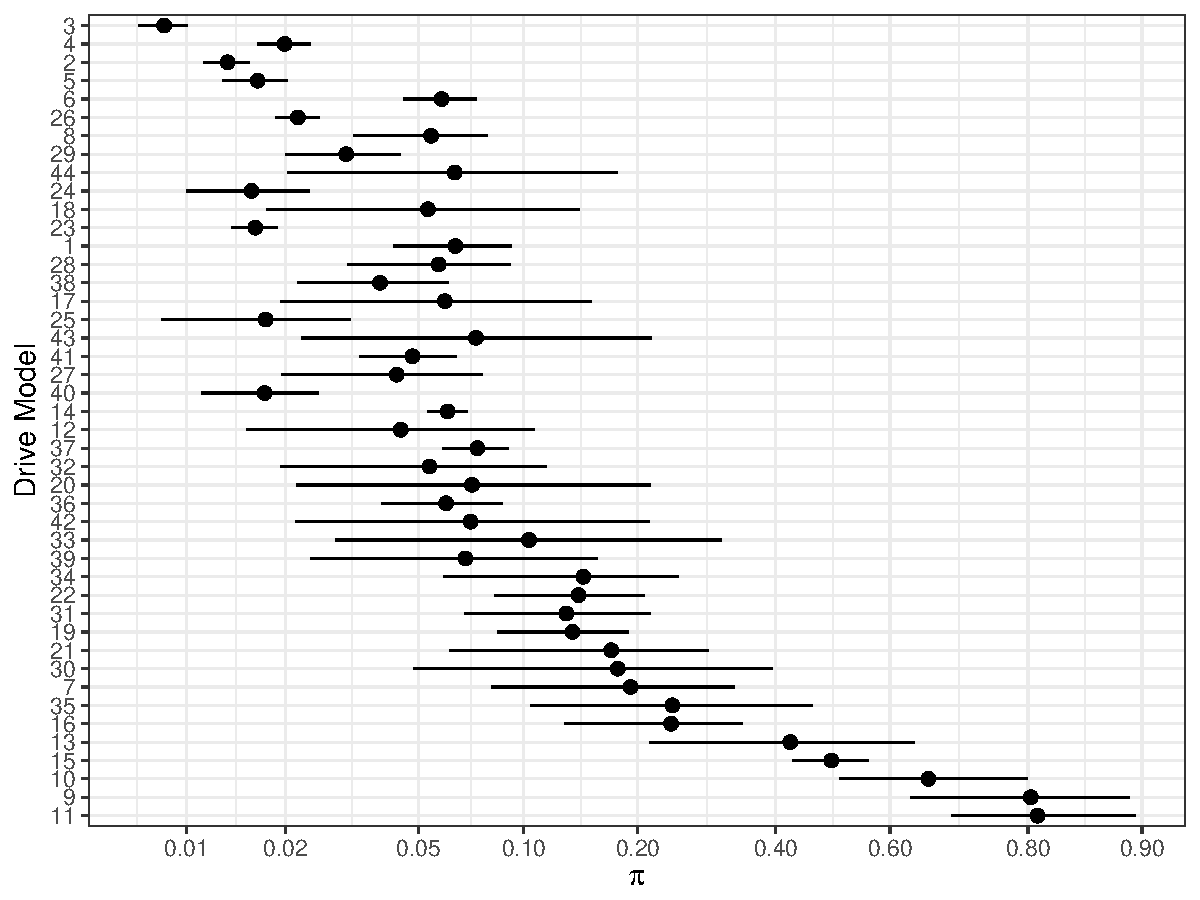
\includegraphics[width=1\linewidth]{pinew.pdf}
   \caption{50\% CI for $\pi$}
   \label{fig:Ng2}
\end{subfigure}

\caption{(a) 50\% CI (in years) for $t_{0.10}$ (b) 50\% CI for $\pi$ plotted on the logit scale.  Both plots are sorted based on the median value of $t_{0.10}$.}
\end{figure}

 
 
%\begin{figure}[H]
  %\centering
  %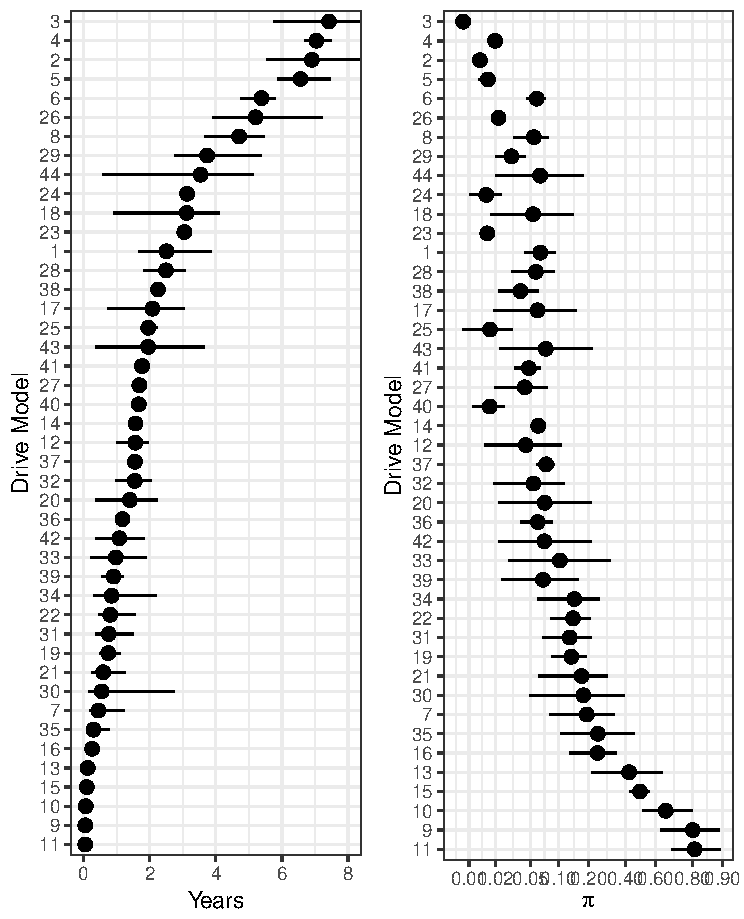
\includegraphics[width=\textwidth]{b10andpi}
  %\caption{Left: 50\% credible intervals for  $t_{0.10}$ (time in years till 10\% of the drives fail). Right: 50\% credible intervals for $\pi$ plotted on the logit scale.  Both plots are sorted based on the median value of $t_{0.10}$.}
  %\label{fig4}
%\end{figure}

\begin{figure}[H]
  \centering
  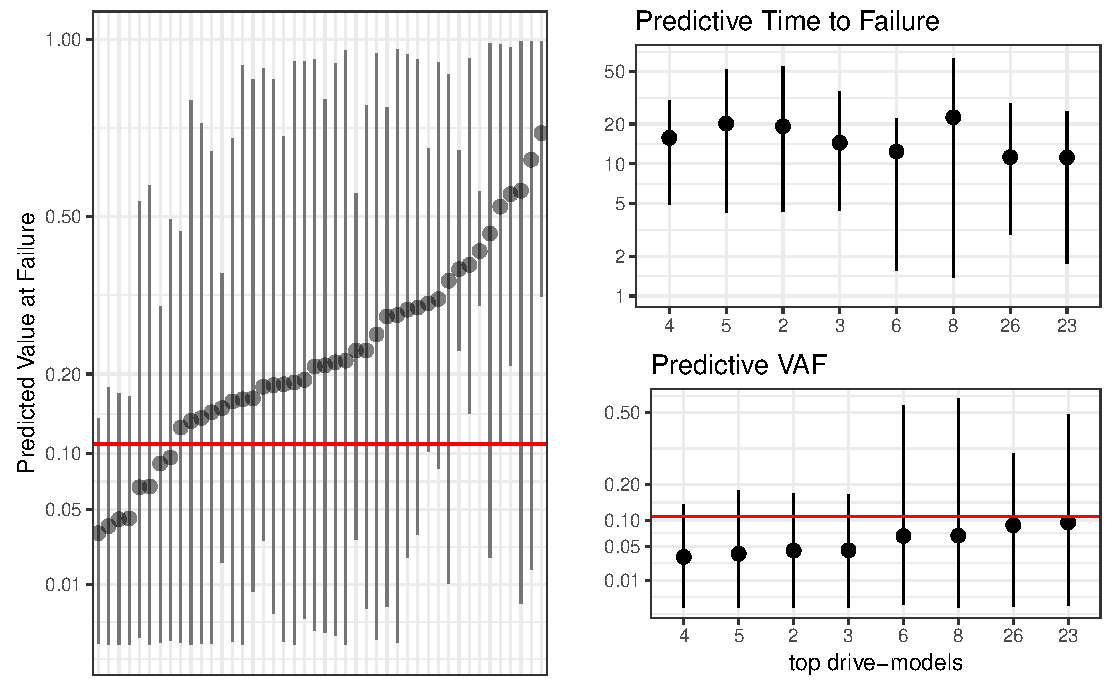
\includegraphics[width=.8\textwidth]{dm-eval}
  \caption{Left: Summary of the posterior predictive distributions for $e^{-0.4 t_{g,new}}$ the depreciated value at failure (VAF) for a new unit for each Drive-model.
  Right: A comparison of the predictive distribution of TTF (top) and VAF (bottom) based on 40\% for best 11 Drive-models, shows that rankings produced by the two measures are not equivalent.}
  \label{fig5}
\end{figure}


\section{Discussion}
\label{sec:Discussion}
This paper offers a new approach to modeling and making inference for the lifetime of consumer products using incomplete field reliability data.  Products with long lifetimes often have few failures and when failures do occur the cause is frequently unknown to the analyst.  The GLFP model provides a framework to accurately model real data with evidence of multiple failure modes. Moreover, when there are multiple product populations within the same product class, our hierarchical modeling approach borrows strength across brands with many observed failures to help make inference for those populations with little information.  This can be important when trying to leverage multiple sources of data with various sample sizes and levels of censoring and truncation.  We found that the use of weakly informative priors on the hyperparameters can increase the overall efficiency of the MCMC. %This makes standard parametric lifetime models inaccurate and difficult to estimate using classical estimation techniques such as ML.  
  
We should point out some important caveats of our analyses, given certain model assumptions. 

First, we assume the failures occurring from various causes can be approximately assigned to two phases of product life.  In practice, there might be additional phases, clearly supported by the data, making the GLFP model too rigid. This rigidity is illustrated by the right tail of the estimated distribution in figure \ref{fig1}. Extrapolations of the fitted model appear to be very conservative and overly confident.

Second, we assume exchangability of units within a population. This assumption is due in part to ignorance about which units are defective but also of potentially important covariates. We do not account for batch effects or varying conditions in the facility which have impacted the observed failure rates. These factors are confounded with Drive-model in our analysis. This second issue is a more fundamental issue with observational data like the hard drive data we have analyzed here.

Consumers of manufactured goods usually lack the data and expertise to perform a failure analysis to determine the cause of failure.  Moreover, their interest is primarily in the lifetime distribution of a product rather than the specific cause of failure.  The ability to fit marginal models, such as GLFP, allow consumers and manufacturers to accurately model products with bathtub hazard lifetime distributions and make comparisons across different product groups.  Because the Bayesian approach provides full posteriors distributions once a model is fit, the analyst can easily estimate a functional, such as a quantile or depreciation factor, that allow products to be compared using statistics meaningful in the context of the data. 

Besides comparing different Drive-models for purchasing decisions, another important application would be prediction of future failures (say, week-by-week) to assure that there is always a sufficient number of replacement drives available.  Methods similar to those in \cite{hmm} can be adapted to Bayesian prediction, as described in Section 15.5 of \cite{intervals}.
 
\section*{Acknowledgment}    
The authors express their gratitude to Dr. \hspace{-.5em} Meeker for his comments and suggestions.

%Hierarchical modeling can be an effective way to regularize a large number of models fits by borrowing information.  %Because all the data contribute some information about the global parameters, it is often sufficient to use weakly %informative priors on the global parameters, making the resulting shrinkage data dependent.  Analysis using HMC is %accessible to practitioners by Stan. HMC has been shown to be very efficient in effective samples per iteration because %its joint updating scheme.  
\clearpage

\appendix
\section{Truncation adjusted nonparametric estimate of lifetime}
\label{sec:trunc-adj}
We first start with a non-parametric estimate of the empirical cdf for each Drive-model using the Kaplan-Meier estimator.  With left truncation, however, the standard Kaplan-Meier estimator for Drive-model $d$, denoted by
$\widehat{F_d(t)}_{KM}$, is conditional on survival up to
$t_{d,\text{min}}^L$, the shortest reported running time of all units
of drive-model $d$ for which records are available. To produce
unconditional estimates, we adapt the adjustment method outlined by \citet[Chapter 11]{meeker}.  For each Drive-model we select
$t_{d,\text{min}}^L$, the smallest left truncated time in the sample.
By sampling from the full posterior distribution, since
$\Pr(T>t_{d,\text{min}}^L|\theta_d)$ (the probability a hard drive has
survived up to $t_{d,\text{min}}^L$) is a function of the model
parameters, we can easily compute its posterior median,
$\widehat{A}_{\text{med}} = \widehat{\Pr}(T>t_{d,\text{min}}^L|\theta_d)$. We compute the adjusted estimate by

$$\widehat{F(t)}_{KMadj} = \widehat{A}_{\text{med}} + \left(1 - \widehat{A}_{\text{med}}\right)\widehat{F_d(t)}_{KM},\; t>t_{d,\text{min}}^L.$$

While this adjustment is negligible for the majority of drive-models, five drive-models receive upward adjustments of greater than 5 percent and the estimated time to failure distribution of one drive-model (30) was adjusted by nearly 16 percent, in part because the shortest truncation time for all observed units was approx. 2.3 years.

\section{Supplementary Material}
\label{sec:supple}

\begin{description}

\item[Stan Code] Stan code for Model 4 (pdf file)

\item[Graphs of Model Comparison Fits for all Drive-models] Posterior median of proportion failing as a function of time under Models 1-4 for all Drive-models. (pdf file)

\item[Posterior Predictive Graphical Checks for all Drive-models] Nonparametric estimates of proportion failing for original and replicated data sets for all Drive-models. (pdf file)

\end{description}


\bibliography{./sample}

\end{document}
